\documentclass[../../InformazioneQuantistica.tex]{subfiles}

\begin{document}

\chapter{Algoritmi quantistici}

\lesson{13 \greendot}{17/4/2019}
Supponendo di riuscire a realizzare fisicamente un computer quantistico, è possibile attuare algoritmi \textit{più efficienti} degli analoghi classici, almeno per certi problemi. Esamineremo alcuni di essi in questa sezione.\\
Al giorno d'oggi, tuttavia, non esiste un \q{compilatore quanti
stico}, ossia un sistema in grado di \q{implementare} un problema classico in un sistema quantistico con un certo guadagno computazionale.

\subsection{Algoritmo di Deutsch}
Consideriamo una \textbf{scatola nera}, ossia un \textit{modulo}, di contenuto ignoto, che prenda un certo input $x$ ($n$ bit) e restituisca un output $f(x)$ (a un solo bit), dove la funzione $f\colon \{0,1\}^n \to \{0,1\}$ - intesa come \textit{deterministica} - appartiene a una delle due classi seguenti:
\begin{itemize}
\item \textbf{Bilanciata}: $f$ mappa metà dei valori possibili di $x$ in $0$ e l'altra metà in $1$. In altre parole, per un $x$ scelto a caso, $f(x)$ è pari a $0$ o a $1$ con la stessa probabilità.
\item \textbf{Costante}: l'output $f(x)$ è sempre pari a un certo valore $k \in \{0,1\}$. In altre parole, $f(x)$ restituisce soli $0$ (o soli $1$) indipendentemente dall'input $x$ inserito.
\end{itemize}
Senza fare ipotesi su come tale scatola nera sia effettivamente realizzata, vogliamo trovare un modo, il più efficiente possibile, per determinare a \textit{quale} delle due classi appartenga $f$.

\textbf{Nota}: una generica funzione $f\colon \{0,1\}^n \to \{0,1\}$ per $n>1$ può non appartenere ad una delle due classi. Perciò funzioni bilanciate o costanti sono classi \q{speciali} di funzioni.\\
Tuttavia, nel caso unidimensionale, con $f\colon \{0,1\} \to \{0,1\}$, vi sono solo $4$ possibilità, $2$ bilanciate e $2$ costanti (tabella \ref{tab:one-bit}).

\begin{table}[H]
\centering
\begin{tabular}{@{}l|rrrr@{}}
\toprule
\multicolumn{1}{c|}{$x$} & \multicolumn{1}{c}{$f_0$} & \multicolumn{1}{c}{$f_1$} & \multicolumn{1}{c}{$f_2$} & \multicolumn{1}{c}{$f_3$} \\ \midrule
0 & 0 & 0 & 1 & 1 \\
1 & 0 & 1 & 0 & 1 \\ \bottomrule
\end{tabular}
\caption{Vi sono solo $4$ funzioni a 1-bit, $2$ bilanciate ($f_1$ e $f_2$) e $2$ costanti ($f_0$ e $f_3$)}
\label{tab:one-bit}
\end{table}

Classicamente, una possibile strategia consiste semplicemente nell'esaminare $f(x)$ per vari valori di $x$. Sono necessari almeno $2$ input per stabilire che $f$ sia bilanciata, dato che basta trovare $x_1$ e $x_2$ t.c. $f(x_1) \neq f(x_2)$. Nel caso $f$ sia costante, tuttavia, servono ben $2^{n-1}+1$ tentativi per averne certezza, dato che una $f$ bilanciata ammette solo $2^{n-1}$ scelte di input che corrispondano allo stesso output.\\
Nel caso quantistico, d'altro canto, l'algoritmo di Deutsch permette di accertare la classe di $f$ esaminando in ogni caso \textit{un solo} output. Vediamo come.\\

Partiamo dal caso (più semplice) di $f: \{0,1\} \to \{0,1\}$, per cui abbiamo già elencato tutte le possibilità in tabella \ref{tab:one-bit}. Consideriamo allora una versione quantistica dell'oracolo, ottenuta sostituendo ai bit $0$, $1$ i qubit $\ket{0}$ e $\ket{1}$ di una opportuna base computazionale (figura \ref{fig:scatola-nera}).\\
Ogni computazione quantistica deve essere \textit{reversibile}. Dobbiamo perciò \textit{portarci dietro} l'input iniziale, come schematizzato in figura \ref{fig:oracolo-quant}.

\begin{figure}[H]
\centering
    \begin{subfigure}[t]{0.45\textwidth}
        \centering
        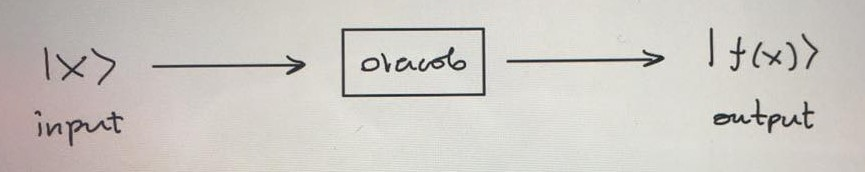
\includegraphics[width=0.7\textwidth]{Immagini/17_4/1.jpg}
        \caption{\footnotesize Schema del funzionamento della \textit{scatola nera} (o oracolo), che \q{applica} una certa funzione $f$ all'input $x$\label{fig:scatola-nera}}
    \end{subfigure}%
    \begin{subfigure}[t]{0.45\textwidth}
        \centering
        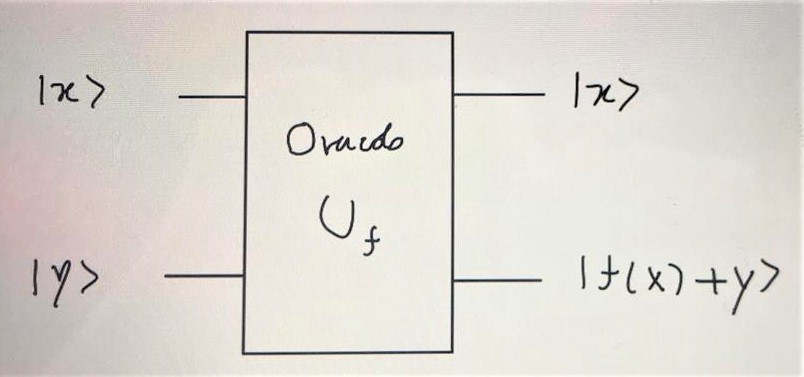
\includegraphics[width=0.7\textwidth]{Immagini/17_4/2.jpg}
        \caption{\footnotesize Funzionamento dell'oracolo quantistico (reversibile)\label{fig:oracolo-quant}}
    \end{subfigure}
\caption{Scatola nera: versione \textit{classica} e \textit{quantistica}}
\end{figure}

L'algoritmo di Deutsch consiste allora nel seguente circuito quantistico:
\begin{figure}[H]
\centering
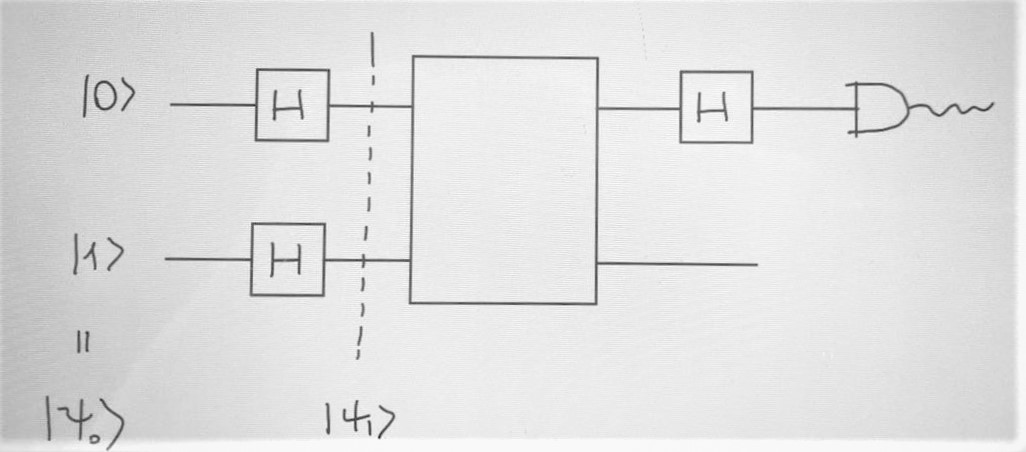
\includegraphics[width=0.7\textwidth]{Immagini/17_4/3.jpg}
\caption{Schema a porte logiche quantistiche dell'algoritmo di Deutsch\label{fig:Deutsch-gates}}
\end{figure}

Esaminiamone il funzionamento. Consideriamo come input iniziale $\ket{\Psi_0} = \ket{0}\ket{1}$.\\
Dopo l'applicazione delle Hadamard otteniamo:
\begin{align*}
\ket{\Psi_1} = (H\otimes H) \ket{\Psi_0} &= \frac{1}{2}(\ket{0}+\ket{1})(\ket{0}-\ket{1}) =\\
&= \frac{1}{2}\ket{0}[\ket{0}-\ket{1}] + \frac{1}{2}\ket{1}[\ket{0}-\ket{1}]
\end{align*}
Ogni Hadamard trasforma un qubit in una sovrapposizione coerente dei due stati possibili. Come vedremo, è proprio questo passaggio che permette al computer quantistico di \textit{esaminare tutti gli input} in una volta sola.\\

Calcoliamo l'azione di $U_f$ su uno stato $\ket{x}[\ket{0}-\ket{1}]$. Ricordando la definizione (figura \ref{fig:oracolo-quant}), per linearità:
\begin{align*}
U_f \ket{x}[\ket{0}-\ket{1}] = U_f \ket{x}\ket{0}- U_f \ket{x}\ket{1} &= \ket{x}\ket{f(x)+0} - \ket{x}\ket{f(x)+1} =\\
&=\ket{x}[\ket{f(x)+0}-\ket{f(x)+1}]
\end{align*}
dove la somma binaria ($+$) è equivalente all'operazione XOR ($\oplus$).\\
Abbiamo due possibilità $f(x)=\pm 1$. Calcoliamole separatamente:
\begin{itemize}
\item Per $\bm{f(x)=0}$:
\begin{align*}
\ket{f(x)+0} -\ket{f(x)+1} = \ket{0}-\ket{1}
\end{align*}
\item Per $\bm{f(x)=1}$:
\begin{align*}
\ket{f(x)+0}-\ket{f(x)+1} =\ket{1}-\ket{0} = -(\ket{0}-\ket{1})
\end{align*}
\end{itemize}
Mettendo tutto insieme:
\begin{align*}
\ket{x}[\ket{0}-\ket{1}] \underset{U_f}{\mapsto} (-1)^{f(x)}\ket{x} [\ket{0}-\ket{1}]
\end{align*}
Possiamo ora calcolare $U_f \ket{\Psi_1}$, sovrapponendo i casi per i due valori di $\ket{x}$:
\begin{align*}
\ket{\Psi_2} &= \frac{1}{2}\big[(-1)^{f(0)} \ket{0}[\ket{0}-\ket{1}] + (-1)^{f(1)}\ket{1}[\ket{0}-\ket{1}]\big] = \\
&= \frac{1}{2}\big[ (-1)^{f(0)} \ket{0} + (-1)^{f(1)} \ket{1}\big]_1 \otimes \big[\ket{0}-\ket{1}\big]_2
\end{align*}
E infine resta da calcolare l'ultimo Hadamard:
\begin{align*}
\ket{\Psi_3} &= (H\otimes \bb{I}) \ket{\Psi_2} = \frac{1}{2\sqrt{2}} \Big [
(-1)^{f(0)} (\ket{0} + \ket{1}) + (-1)^{f(1)} (\ket{0}-\ket{1}) 
\Big ]_1 \otimes \Big[ \ket{0} - \ket{1} \Big]_2 = \\
&= \frac{1}{2\sqrt{2}} \Big[\big((-1)^{f(0)} + (-1)^{f(1)}\big) \ket{0} + \big((-1)^{f(0)} - (-1)^{f(1)} \big)\ket{1}\Big]_1 \otimes \Big[\ket{0}-\ket{1}\Big]_2
\end{align*}
A questo punto misuriamo lo stato del primo qubit, che sarà $\ket{0}$ o $\ket{1}$ con probabilità date dal modulo quadro dei rispettivi coefficienti. Ma se $f(0)=f(1)$ (funzione costante) si ha che $\ket{1}$ ha probabilità nulla, mentre se $f(0)\neq f(1)$ (funzione bilanciata) stavolta $\ket{0}$ ha probabilità nulla. Perciò, in un caso o nell'altro, troveremo \textbf{un solo risultato} con certezza - cosa che ci permette di distinguere da \textit{una sola misura} la classe della funzione $f$.\\

Generalizziamo tutto ciò al caso di $f$ (bilanciata o costante) che prende in input $n$ qubit:
\begin{align*}
f:\{0,1\}^n \to \{0,1\}
\end{align*}
Lo stato di partenza è, in questo caso, pari a:
\begin{align*}
\ket{\Psi_0} = \underbrace{\ket{0}\ket{0}\cdots \ket{0}}_{n}\ket{1}
\end{align*}
Estendendo il circuito visto in figura \ref{fig:Deutsch-gates} (che ora è detto algoritmo di Deutsch-Jorza), ciascuno degli $n+1$ input viene mandato in una Hadamard, dopo le quali otteniamo un nuovo stato:
\begin{align*}
\ket{\Psi_1} &= (H^{\otimes n} \otimes H) \ket{\Psi_0} = \frac{1}{\sqrt{2^n}} \left(\sum_{x=0}^{2^n-1}\ket{x}_n\right) \frac{(\ket{0}-\ket{1})}{\sqrt{2}}
\intertext{dove con $\ket{x}_n$ si intende lo stato di $n$ qubit $\ket{x_0}\ket{x_1}\ket{x_2}\otimes \dots \otimes \ket{x_{n-1}}$, con $x_i$ $i$-esima cifra binaria di $x$.}
\intertext{L'estensione naturale dell'azione dell'oracolo a più qubit risulta in:}
\ket{\Psi_2} &= U_f \ket{\Psi_1} =  \frac{1}{\sqrt{2}}\frac{1}{\sqrt{2^n}} \sum_{x=0}^{2^n-1}(-1)^{f(x)} \ket{x}_n (\ket{0}-\ket{1})_{n+1}
\intertext{dove con $\ket{x}_n$ si intende lo stato dei primi $n$ qubit, con la conversione di $x$ da decimale a binario. Per esempio, per $n=3$, $\ket{3}=\ket{011}_3$. L'ultimo ket, d'altro canto, riguarda solo l'$n+1$-esimo qubit.}
\intertext{Applichiamo ora $n$ Hadamard a tutti gli input tranne l'$n+1$-esimo, ottenendo:}
\ket{\Psi_3} &= (H^{\otimes n} \otimes \bb{I}) \ket{\Psi_2} = \frac{1}{2^n}\Big[ \sum_{x,y=0}^{2^n-1} (-1)^{f(x)+x\cdot y} \ket{y} \Big]_n \otimes \frac{1}{\sqrt{2}} \Big[ \ket{0} - \ket{1} \Big]_{n+1}
\intertext{dato che:}
H^{\otimes n}\ket{x} &= \prod_{i=0}^{n-1}\left( \frac{1}{\sqrt{2}} \sum_{y_i=0}^1 (-1)^{x_i y_i}\ket{y_i} \right) = \frac{1}{\sqrt{2^n}} \sum_{y=0}^{2^n -1} (-1)^{x\cdot y} \ket{y}
\intertext{dove $x\cdot y$ è il prodotto scalare tra i bit di $x$ e $y$ (che ha parità ben definita).}
\end{align*}

Misuriamo ora i primi $n$ qubit (l'$n+1$-esimo può essere scartato).\\
Di nuovo, avremo due casi:
\begin{itemize}
\item Per $f(x)=\text{costante}$ vi è un solo stato finale possibile:
\begin{align*}
\ket{\Psi_4} = \underbrace{\ket{0}\cdots \ket{0}}_{n} (\ket{0}-\ket{1})_{n+1}
\end{align*}
Per esempio, supponiamo $f(x) \equiv 0$. Allora lo stato dei primi $n$ qubit prima della misura è:
\begin{align*}
    \ket{\Psi_3}_n = \frac{1}{2^n} \sum_{x,y=0}^{2^n-1} (-1)^{x\cdot y} \ket{y} 
\end{align*}
La probabilità che $\ket{0\cdots 0}_n$ venga selezionato è data dal modulo quadro del braket:
\begin{align*}
\braket{\Psi_3|0\cdots 0} = \frac{1}{2^n} \sum_{x=0}^{2^n-1}(-1)^0 \braket{0\cdots 0|0\cdots 0} = 1
\end{align*}
dove abbiamo usato l'ortonormalità dei vettori della base computazionale. Poiché la probabilità di tale stato \textit{esaurisce} tutte le possibilità, tale stato è l'unico possibile. Lo stesso risultato si ottiene nel caso sia $f(x) \equiv 1$, dove il braket è $-1$, ma ciò non cambia il suo modulo quadro (la probabilità), che è sempre pari a $1$ (certezza).

\item Per $f(x)$ bilanciata, invece, la probabilità di ottenere $\ket{0\cdots 0}_n$ è identicamente nulla, dato che:
\begin{align*}
    \braket{\Psi_3|0\cdots 0} = \frac{1}{2^n} \sum_{x=0}^{2^n-1} (-1)^{f(x)} = \frac{1}{2^n} \left[ (-1)^{f(0)} + (-1)^{f(1)} + \dots + (-1)^{f(2^n-1)} \right ]
\end{align*}
e $f(x) = 0$ esattamente metà delle volte, e pari a $1$ altrimenti. Si ottiene perciò una somma di $2^n/2$ termini $+1$ e altrettanti termini $-1$, che porta chiaramente a $0$.\\
Ogni altro stato $\ket{\phi_n} \perp \ket{0\cdots 0}$ è possibile, e perciò lo stato dopo la misura sarà uno di questi:
\begin{align*}
\ket{\Psi_4} = \ket{\phi}_n (\ket{0}-\ket{1})_{n+1}
\end{align*}
\end{itemize}
Perciò un computer quantistico è in grado, con una sola misura, di distinguere la classe della funzione.\\

\textbf{Nota}: il problema appena esaminato richiede $2^{n-1}+1$ misure classiche, o una sola misura quantistica. Il guadagno computazionale, nel caso quantistico, sembrerebbe esponenziale.\\
In realtà stiamo ignorando un fatto importante: $2^{n-1}+1$ misure classiche sono richieste nel caso \textit{peggiore}. In generale, se immaginiamo che gli input $x$ siano mappati \q{uniformemente} a $0$ e $1$, le prime $2^{n-1}$ misure producono lo stesso output solo in due casi su $2^n$, ossia con probabilità $2^{-n+1}$. Mediamente, perciò, sono richieste \textit{molte meno} misure classiche per poter discriminare la classe di $f$, ma comunque almeno $2$. In ogni caso, perciò, l'algoritmo di Deutsch permette un significativo guadagno computazionale (nell'ipotesi che la \textit{black-box} sia implementata efficientemente).

\subsection{Algoritmo di Grover}
Un altro problema che può essere risolto in maniera efficiente da un computer quantistico è la ricerca in un database non strutturato.\\

Possiamo schematizzare un semplice \textbf{database} come un set $A$ di \textit{stringhe} indicizzate dalla loro \textit{posizione}, ossia una mappa $g\colon \bb{N} \supset U \to A$. Il database si dice \textit{strutturato} se gli indici rispettano una relazione d'ordine su $A$, ossia se esiste un modo per \textit{comparare} le stringhe e vale:
\begin{align*}
    x_1 \leq x_2 \Rightarrow U, g(x_1) \leq g(x_2) \qquad \forall x_1, x_2 \in U
\end{align*}
In un database non strutturato, d'altro canto, non esiste alcuna relazione di questo tipo, e l'associazione $x\mapsto g(x)$ è completamente arbitraria.\\
Data una stringa $a \in A$, vorremmo trovare un modo efficiente per trovare il suo indice $x_a \in U$ tale che $g(x_a) = a$.\\
In un \textbf{database strutturato} ciò si può fare con l'algoritmo classico di \textit{bisezione}:
\begin{enumerate}
    \item Si esamina la stringa $a_1 = g(x_1)$ nella posizione $x_1$ centrale del database. Se $a_1 = a$ la ricerca è terminata.
    \item Se $a \neq a_1$, si esamina l'ordine relativo tra $a$ e $a_1$. Se $a$ è a destra della stringa centrale $a_1$, allora sappiamo per certo che l'indice cercato è $>x_1$, e quindi compreso nella metà destra del database. Analogamente, se $a < a_1$, l'indice sarà nella metà sinistra.
    \item Si esamina la stringa corrispondente all'indice intermedio della metà precedentemente considerata. Reiterando gli ultimi due punti è possibile \textit{dimezzare} di volta in volta la regione da esaminare, e dopo pochi passaggi ($O(\log_2 N)$) si giunge alla soluzione.
\end{enumerate}
D'altro canto, la ricerca in un \textbf{database non strutturato} è decisamente meno efficiente. L'unico modo è infatti procedere \textit{sequenzialmente}, e in media dovremo esaminare $N/2$ casi. L'algoritmo è quindi di ordine $O(N/2)$.\\

Quantisticamente, l'algoritmo di Grover permette un guadagno \textit{quadratico}, passando da $O(N)$ a $O(\sqrt{N})$. Vediamo come.\\

Ridefiniamo il problema in termini di qubit. Sia $\bar{x}$ la posizione cercata (vista come stringa di $n$ bit). Definiamo una funzione $f(x)$ (detta \textit{oracolo}) che indichi se una posizione $x$ esaminata è proprio quella $\bar{x}$ della stringa cercata:
\begin{align*}
f(x):\{0,1\}^n \to \{0,1\} \qquad f(x) = \begin{cases}
1 & x = \bar{x}\\
0 & x \neq \bar{x}
\end{cases}
\end{align*}
La ricerca di una stringa è quindi equivalente a trovare l'unico valore $\bar{x}$ (tra tutti gli indici $x$ possibili) tale che $f(\bar{x}) = 1$.\\

Supponiamo, per semplicità, di avere indici di $2$ qubit, per un totale di $2^2 = 4$ possibili entrate nel database. In tal caso, l'algoritmo di Grover è implementato dal circuito di figura \ref{fig:Grover-gates}. 

\begin{figure}[H]
\centering
\begin{quantikz}
\lstick[wires=2]{$\ket{00}$}\slice{$\ket{\Psi_0}$} & \gate{H} \slice{$\ket{\Psi_1}$} & \gate[wires=3][1.7cm]{U_f}\gateinput[2]{$x$}
\gateoutput[wires=2]{$x$} \slice{$\ket{\Psi_2}$} &  \qw  & \gate{H}\gategroup[2,steps=7,style={dashed, rounded corners, fill=blue!20, inner xsep=2pt}, background]{{D}} & \gate{\sigma_x} & \qw & \ctrl{1} & \qw & \gate{\sigma_x} &  \gate{H}  & \qw \rstick[wires=2]{$\ket{\bar{x}}$} \\
& \gate{H} & \qw & \qw & \gate{H} & \gate{\sigma_x} & \gate{H} & \targ{} & \gate{H} & \gate{\sigma_x} & \gate{H} & \qw\\
\lstick{$\ket{1}$} & \gate{H} & \gateinput{$y$}\gateoutput{$y \oplus f(x)$} & \qw & \qw & \qw & \qw & \qw & \qw & \qw & \qw & \rstick{$\frac{1}{\sqrt{2}}(\ket{0}-\ket{1})$} \qw
\end{quantikz}
\caption{Schema in porte logiche quantistiche dell'algoritmo di Grover per indici a $2$ qubit\label{fig:Grover-gates}}
\end{figure}



\begin{comment}
Domanda: si può estendere l'algoritmo di Deutsh anche a funzioni bilanciate "probabilistiche", definite come:
f:\{0,1\}^n \to \{0,1\}
e tali che f(x) = 0 con p=0.5 e f(x) = 1 con p=0.5
\end{comment}


\end{document}

